\documentclass[a4paper,twocolumn,fleqn]{article}
\textwidth 17cm \textheight 247mm
\topmargin -4mm
\hoffset -9mm \voffset -14mm
%\setlength{\topmargin}{-0.8truecm}
\setlength{\oddsidemargin}{0.3cm}
\setlength{\evensidemargin}{0.3cm}
\setlength{\columnsep}{8mm}
\setlength{\parindent}{0mm}
\setlength{\parskip}{-2.0ex}
\setlength{\mathindent}{0mm}
\flushbottom


\usepackage{epsfig}
%\usepackage{timesnew}
% \usepackage{harvard}
\usepackage[]{natbib}
\usepackage{amsmath}
\usepackage{booktabs}

\usepackage[latin1]{inputenc}
\usepackage{aeguill}
\usepackage[frenchb,english]{babel}
\usepackage{caption}


\setlength{\parskip}{2ex} \pagestyle{myheadings}
\markright{\hspace*{3.8cm} \textit{MOSIM18 - June 27-29, 2018 - Toulouse - France}}

\renewcommand{\thepage}{}
\renewcommand{\refname}{REFERENCES}



\makeatletter
\renewcommand\section{\@startsection{section}{1}{\z@}%
                       {-6\p@ \@plus -0\p@ \@minus -0\p@}%
                       {2\p@ \@plus 0\p@ \@minus 0\p@}%
                       {\normalsize\textbf}}

\renewcommand\subsection{\@startsection{subsection}{2}{\z@}%
                       {-6\p@ \@plus -0\p@ \@minus -0\p@}%
                       {2\p@ \@plus 0\p@ \@minus 0\p@}%
                       {\normalsize\textbf}}

\renewcommand\subsubsection{\@startsection{subsubsection}{3}{\z@}%
                       {-6\p@ \@plus -0\p@ \@minus -0\p@}%
                       {1\p@ \@plus 0\p@ \@minus 0\p@}%
                       {\normalsize\itshape\bfseries}}
\makeatother


\begin{document}

\title{ \vspace*{-25mm}
\centering
\fbox{\normalsize
\begin{minipage}{17cm}
\centering
\em \small{$12^{th}$ International Conference on MOdeling, Optimization and SIMlation - MOSIM18 - June 27-29 2018  \\ Toulouse - France "The rise of connected systems in industry and services"}
\end{minipage} }\\
\vspace*{6mm}
{\Large \textbf{Bi-objective MIP formulation for the optimization of maintenance planning on French military aircraft operations}}}

\author{
\begin{tabular}{c}
\bf \normalsize {Franco Peschiera, Alain Ha�t, Olga Batta�a, Nicolas Dupin} \\
\\
     \normalsize ISAE-SUPAERO, % \\
     \normalsize Universit� de Toulouse, % \\
     \normalsize 31055 Toulouse cedex 4 - France\\
     \normalsize {\{franco.peschiera,alain.hait,olga.battaia,nicolas.dupin\}@isae-supaero.fr}
     \\
\end{tabular}
}

\date{\begin{minipage}{17cm}
\normalsize
{\bf  ABSTRACT:}
\rm
{\em A specific Flight and Maintenance Planning problem is presented. 
In this problem, preventive maintenance operations are scheduled for military aircraft along with the assignment of regular missions. 
The quality of the solutions is measured via a bi-objective function that smooths both maintenance operations and aircraft unavailability among time periods. 
An exact optimization approach is provided by a Mixed Integer Programming model.
A real world dataset provided by the French Air Force is used to test the developed optimization approach.
Mono-objective computations are solved to optimality for medium size instances, allowing to compute exactly the Pareto frontier of the bi-objective optimization problems.
The tests show that these two objectives do not lead to the same optimal solution, but very good compromise solutions can be found thanks to the bi-objective optimization.
}\\~\\
{\bf KEYWORDS:}
\rm
{\em optimization, Flight and Maintenance Planning, aircraft maintenance, Mixed Integer Programming, bi-objective optimization}
\end{minipage}
}
\maketitle

% Here I put the list of things we will leave for another article:
% 1. stochasticity
% 2. symmetry breaking inside model.
% 3. storage?

\section{Introduction}
  
  Flight and Maintenance Planning (FMP) problems are raised in civilian or military operational applications. 
  They schedule maintenances of aircraft taking into account the implications of maintenance immobilizations for the demand in flight hours, for a conjoint optimization among maintenance dates and flight hours.

  The specific FMP of this paper comes from the French Air Force's operations. It has two specificities regarding the classical FMP considered in the literature.
  On one hand, the fleet of aircraft is heterogeneous, with different standards, capacities and retrofits.
  On the other hand, there is a will to align two objectives: the smoothing of the maintenance operations and the minimization of the global unavailability of aircraft to be able to add new missions. This last point calls for a bi-objective optimization.

  This paper investigates how to solve such new optimization problem, and how to take good compromise decisions if these objectives are antagonistic.

  The article is structured as follows:

  Section \ref{sec:problem} presents a detailed description of the problem. An analysis of the previous work on FMP is given in section \ref{sec:soa}.
  Section \ref{sec:model} presents a new MIP formulation for the considered problem. 
  Section \ref{sec:data} introduces the real case study.
  Section \ref{sec:results} discusses the obtained results.
  Finally, section \ref{sec:conclusions} provides conclusions and directions of further work.

\section{Problem statement}
  \label{sec:problem}
  The problem consists in assigning resources to predefined tasks and scheduling periodic preventive maintenances for these same resources. For the seek of simplicity, the following convention has been adopted: aircraft are called resources, missions are called tasks.

  \subsection{Tasks}
    \label{def:task}

    There is a fixed set of $j \in \mathcal{J}$ tasks to be accomplished over an horizon of time divided into $t \in \mathcal{T}$ discrete periods. For their execution, these tasks require the assignment of a specific number of resources $R_j$ each period of time the task is active. The start and end periods for each task are known and a task is considered active between its start and end period.
    
    During each period, tasks consume an amount of time equal to $H_j$ from each of its assigned resources.

    % The assignment of a resource to a task is not decided for the whole duration of the task. After a minimum amount of time ($MT$), a resource can be freed and exchanged for another one, even if the task it is assigned to has not finished. 
    The total number of resources being used at any given time in a specific task should be equal to $R_j$.

    Each task requires one and only one type of resource which, in addition, should comply with additional task requirements.

  \subsection{Resources}
    \label{def:res}

    There is a set $i \in \mathcal{I}$ of available resources that are assigned to tasks in order to accomplish them. Each resource can only be assigned to a single task in any given period. These resources suffer from wear and tear and require regular maintenance operations during their lifetime. The need for maintenance is calculated based on two indicators.
    
    The first one is called "remaining elapsed time" (or $ret_{it}$). It expresses the amount of time (measured in time periods) after which the resource cannot be used anymore and has to undergo a maintenance operation. Its value is calculated for each resource $i$ and each time period $t$. In a similar way, "remaining usage time" (or $rut_{it}$) is used to measure the amount of time that the resource $i$ can be used before needing a maintenance operation at any given period $t$.

    % Additionally, after an absolute amount of time and/or usage ($aet_i$ or $aut_i$), the resource becomes obsolete. There is no way to reverse this process.

    At any given period, including at the start of the planning horizon, each resource has a specific status given by remaining usage time and remaining elapsed time.

    % \begin{itemize}
        % \item remaining absolute elapsed time.
        % \item remaining absolute usage time.
        % \item remaining storage time (see \ref{def:sto}).
        % \item type of last maintenance (see \ref{def:maint}).
    % \end{itemize}


  \subsection{Maintenances}
    \label{def:maint}

    Maintenances operations are the process by which resources that have reached a limit in some indicator can return to a state where they can continue to be used in tasks.

    % Each maintenance belongs to a specific type of maintenance $m \in \mathcal{M}$. These types of maintenance differentiate between each other by having potentially different characteristics such as: different durations, the provision of new functionalities for the resource or the restoration of the storage capacity (see \ref{def:sto}). The maintenance type is not a decision to be made since there is a specific sequence of maintenance types a resources needs to follow according to the resource type.

    Each maintenance operation has a fix duration of $M$ periods.

    After a maintenance operation, a resource restores its remaining elapsed time and remaining usage time to their max values $E$ and $H$ respectively.

    % Finally, resources are organized into families or groups. Each resource inside a family or group shares the same types of maintenances and, usually, is able to do the same type of tasks.

  % \subsection{Storages}
  %   \label{def:sto}

  %   Following the rule of remaining elapsed time, even if a resource is not being used, it still needs to have a maintenance after a given amount of time has passed. In order to avoid this problem, the resource can be put into a storage state.

  %   A resource in this states has to be kept for a minimum time of $sm$ periods. While in this state it cannot receive maintenance or be assigned any task.

  %   Every resource has the capacity to be stored and this capacity is measured in a number of periods $sc$. In order for a resource to restore its remaining storage capacity, it needs to receive a specific maintenance (see \ref{def:maint}). Similar to the remaining elapsed time, after these maintenances, the resource recovers its storage capacity up to a certain level $S$.

  \subsection{Possible states}

    As a summary, the following are the possible logical states that a resource can be in: assigned to a task (see \ref{def:task}); under maintenance (see \ref{def:maint}); available.

      % \begin{itemize}
          % \item Under storage (see \ref{def:sto}).
            % \item Obsolete (see \ref{def:res}).
      % \end{itemize}


    % Figure \ref{fig:solution} shows an extraction of an assignment of missions (red) and maintenances (blue) to aircraft (codes A1 - A9).

    %   \begin{figure}
    %     \centering
    %       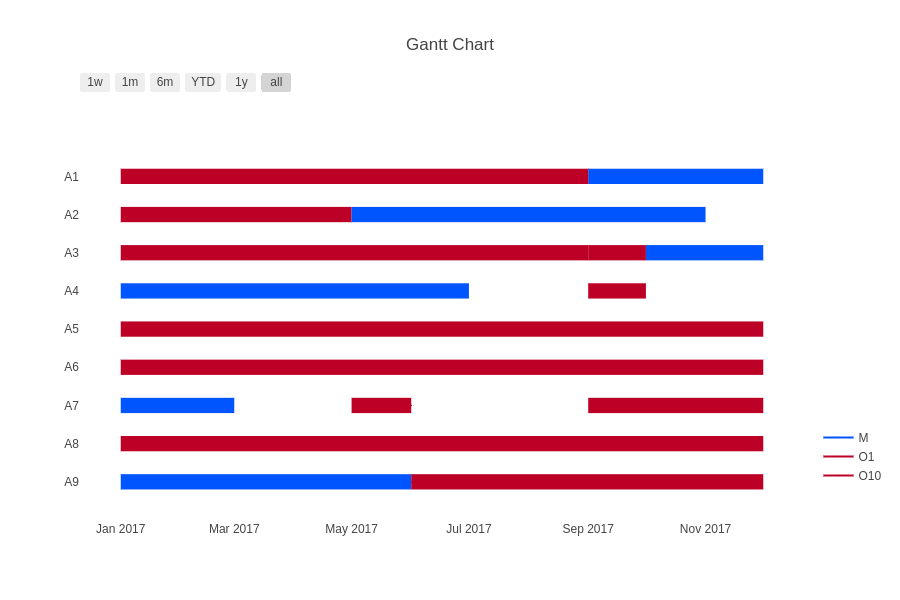
\includegraphics[width=0.5\textwidth]{./../../img/calendar.png}
    %     \caption{Visual representation of part of the solution to an instance of the problem showing maintenances and assignments. Resources are listed in the vertical axis and the horizontal axis defines the time. Red periods correspond to task assignments while blue ones to maintenance assignments.}
    %     \label{fig:solution}
    %   \end{figure}
    

  \subsection{Time}
    \label{def:hor}

    In planning tasks and maintenances, it is important to take into account the initial and end state of each resource. This initial state can be a maintenance or an assigned task. If a resource is under maintenance, it needs to continue in this state for its remaining maintenance time. Tasks' assignments should be taken into account in a similar manner.

    The remaining used and elapsed times are assigned to each resource at the beginning of the planning horizon.

    Finally, the state of each resource at the end of the planning horizon, its remaining (elapsed, used) time, needs to be defined.
      % needs to be addressed too. This implies guaranteeing that the remaining (elapsed, used) time of resources is sustainable for future tasks and the final states of resources are not too skewed.
  
  \subsection{Objectives}
    
    In this study, the following objectives are considered.

    Given that the creation of new tasks and the duration of maintenance are considered stochastic in real-life, one basic goal is to maximize the robustness of the planning by having the greatest amount of available resources at every period of the planning horizon. 

    Given the limited amount of maintenance capacity and its cost, another goal is to smooth as much as possible the number of resources under maintenance over the planning horizon.

    As it will be shown in the mathematical formulation, these objectives are quite related one with the other: the more resources are in maintenance in a given period, the more unavailable resources will be had.

\section{Related work}
  \label{sec:soa}

  % TODO: add FMP biblio?

  % The Military Flight and Maintenance Planning Problem considered here aims to assign missions and maintenance tasks to military aircraft. It is a variant of the Flight and Maintenance Planning problem where flights are not modeled geographically since a round-trip to the base is assumed for each flight.

  % It also includes different objectives and constraints. 

  % Although the former has been studied in literature in \citet{Cho2011,Chastellux2017,Kozanidis2008,Verhoeff2015}, it has not received as much attention as the latter. In the following, the problem with already scheduled missions is considered.

  The Military Flight and Maintenance Planning problem considered assigns missions and schedules maintenance operations to aircraft. In this problem, aircraft are needed to comply with a series of planned missions while at the same time needing to receive frequent preventive maintenances in order to be ready for new missions.

  It is a variant of the Flight and Maintenance Planning problem, where maintenance operations and flights are scheduled to commercial aircraft. The main differences are the fact that flights are not modeled geographically: all aircraft are assumed to exit the main depot and return to the same depot at the end of the flight.

  Other differences include the following.

  Firstly, the objective function's motivation is on reducing the load on the maintenance facilities and guaranteeing the availability of the fleet instead of reducing the cost. Also, the maintenance operations take considerably longer and the rules that govern the maintenances are different.

  The temporal scope of the problem is also larger, making the normal planning horizon and each period larger too: years instead of months and months instead of days, respectively.

  In the following, the studies on the Military Flight and Maintenance Planning are discussed.

  In \citet{Kozanidis2008}, a model for the Hellenic Air Force is presented. It assigns flight hours to aircraft and schedules flexible maintenance periods based on a "remaining usage time" rule. The objectives are to maximize this "remaining usage time" for the aircraft as well as to smooth the availability of aircraft during the planning horizon. Instances of 24 aircraft and 6 monthly periods were solved with Mixed Integer Programming (MIP) formulations and heuristics.

  In \citet{Cho2011}, the objective is to smooth the maintenance operations. Randomly generated instances of 15 aircraft and 520 bi-daily periods were solved with MIP formulations. The final state of aircraft is taken into account in order to distribute as much as possible the "remaining usage time" of aircraft.

  In \citet{Verhoeff2015}, a model for the Royal Netherlands Air Force is developed. Here, three criteria for improving the planning robustness are presented and applied in a MIP model: availability, serviceability and sustainability.

  In \citet{gavranis2015exact}, an exact algorithm is presented and tested on instances of 6 periods and between 10 and 200 aircraft for the special case of maximizing the residual flight time availability or total remaining usage time. 

  Both \citet{Kozanidis2008} and \citet{Cho2011} develop heuristic alternatives to the MIP formulation for solving larger problem instances. In \citet{steiner2006heuristic}, a constructive, multi-stage heuristic approach is described to obtain balanced maintenances for the Swiss Air Force. Both calendar-based maintenances actions (CBMA) and usage-based maintenance actions (UBMA) are used. Finally, in \citet{kozanidis2014heuristics}, two heuristics are presented to solve large instances of the problem by taking consecutive decisions period by period with the help of mathematical models at each step.

  % Regarding operational-level planning, a more detailed implementation can be found in \citet{safaei2011workforce}, where the specific conditions during the maintenance operations are taken into account to schedule the maintenance jobs, such as the workforce skills and availability.

  It should be noted that previous formulations only consider an aggregate demand in flight hours for all aircraft.
  The aircraft are assumed to be homogeneous and interchangeable.
  The use of aggregate demand makes it impossible to take into account the task requirements for aircraft.
   % The concept of mission is not introduced as part of these formulations, only a demand of flight hours is given for all aircraft in total. The aircraft themselves have been assumed as homogeneous and interchangeable. Due to this aggregation of demand, there are no minimal time assignments for aircraft to missions. Missions are important in order to guarantee that aircraft have the required capabilities needed for the missions they are assigned to.

  % Additionally, the possibility of storage of aircraft is not present in the previous work.

  Lastly, in \citet{Chastellux2016} a mission-centered modeled is presented. Here, cycles, composed of one maintenance followed by mission assignments were used. Instances of 6 - 70 aircraft and 60 monthly periods were solved. Close to optimal solutions for small to medium instances using MIP formulations and heuristics based on these MIP formulations were found.

  In the following, an alternative model is presented. This model is then tested in a case study.

\section{Optimization model}
  \label{sec:model}

  \subsection{Sets}

    \begin{tabular}{p{5mm}p{70mm}}
        % $\mathcal{I}$     &   \\
        % $\mathcal{T}$     &   \\
        % $\mathcal{J}$     &   \\
        $\mathcal{T}_j$     &  time periods $t \in \mathcal{T}$ in which task $j$ is active. \\
        $\mathcal{J}_t $    &  tasks $j \in \mathcal{J}$ to be realized in period $t$. \\
        $\mathcal{I}_j$     &  resources $i \in \mathcal{I}$ that can be assigned to task $j$. \\
        $\mathcal{O}_i$     &  tasks $j \in \mathcal{J}$ for which resource $i$ can be used. \\
        $\mathcal{T}^{s}_t$ &  time periods $t' \in \mathcal{T}$ such that $t' \in \{ \max{\{1, t - M+1\}},  ..., {t}$\}. \\
    \end{tabular}

  \subsection{Parameters}

    \begin{tabular}{p{8mm}p{67mm}}
        $H_j$             & amount of resource time required by task $j$. \\
        $R_j$             & number of resources required by task $j$. \\
        % $MT$              & minimum number of periods a resource can be assigned to a task. \\
        % $aut_i$           & maximal absolute usage time for resource $i$. \\
        % $aet_i$           & maximal absolute elapsed time for resource $i$. \\
        $M$               & maintenance duration in number of periods. \\
        $E$               & remaining elapsed time after a maintenance. \\
        $H$               & remaining usage time after a maintenance. \\
        % $S$               & remaining storage time after (certain) maintenances. \\
        $W_1$             & weight of the first objective in the objective function. \\
        $W_2$             & weight of the second objective in the objective function. \\
        $N_t$             & number of resources in already-planned maintenances in period $t$ at the beginning of the planning horizon.\\
        $D_t$             & number of resources to be assigned in total in period $t$. \\
        $Rut^{Init}_{i}$  & remaining usage time for resource $i$ at the start of the planning horizon. \\
        $Ret^{Init}_{i}$  & remaining elapsed time for resource $i$ at the start of the planning horizon. \\
        $Ret^{Init}_{sum}$& sum of remaining elapsed times at the start of the planning horizon. \\
        $Rut^{Init}_{sum}$& sum of remaining elapsed time at the start of the planning horizon. \\
    \end{tabular}

  \subsection{Variables}

     The following decision variables define a solution.
    
    \begin{tabular}{p{8mm}p{67mm}}
        $a_{jti}$   &  =1 if task $j \in J$ in period $t \in \mathcal{T}_j$ is realized with resource $i \in \mathcal{I}_j$, 0 otherwise. \\  
        $m_{it}$    &  =1 if resource $i \in I$ starts a maintenance operation in period $t \in \mathcal{T}$, 0 otherwise. \\
        $rut_{it}$  &  remaining usage time (continuous) for resource $i \in I$ at the end of period $t \in \mathcal{T}$. \\  
        $ret_{it}$  &  remaining elapsed time (integer) for resource $i \in I$ at the end of period $t \in \mathcal{T}$. \\  
        $u_{max}$   &  maximal number (integer) of unavailable resources in any period. \\
        $m_{max}$   &  maximal number (integer) of resources in maintenance in any period. \\
    \end{tabular}
    
    Note that  $a_{jti}$ and $m_{it}$ are initially set up to 0 for all resources already in maintenance at the beginning of the planning horizon for the remaining time periods of maintenance. The remaining usage time for each resource at the beginning of the planning horizon is used to initialize $rut_{i0}$. 

  \subsection{Constraints}

    The objective is to simultaneously minimize the maximum number of maintenances and the maximum number of unavailable aircraft. 

    \begin{align}
        & \text{Min}\; W_1 m_{max} + W_2 u_{max}
    \end{align}
    where weights $W_1$ and $W_2$ are chosen by the decision maker. 
    The following constraints are used in the model:       
    \begin{align}
        % maximum capacity1:
        & \sum_{t' \in \mathcal{T}^{s}_t} \sum_{i \in \mathcal{I}} m_{it'} + N_t \leq m_{max}
          & t \in \mathcal{T} \label{eq:capacity1}\\
               % maximum capacity2:                
        %        & \sum_{t' = t - m+1}^{t} \,\, \sum_{i \in \mathcal{I}} m_{it'} \leq m_{max}
        % & t =m, ..., |\mathcal{T}|  \label{eq:capacity2}\\
               %avail
       & \sum_{t' \in \mathcal{T}^{s}_t} \sum_{i \in \mathcal{I}} m_{it'} + N_t \notag \\
           &\hspace*{10mm}+ D_t\leq u_{max} 
        &t \in \mathcal{T} \label{eq:avalaibility1}\\
               % maximum capacity2:                
        %        & \sum_{t' = t - m+1}^{t} \,\, \sum_{i \in \mathcal{I}} m_{it'} + D_t\leq u_{max} 
        % & t =m, ..., |\mathcal{T}|  \label{eq:avalaibility2}\\
        & \sum_{i \in \mathcal{I}_j} a_{jti} = R_j
                & j \in \mathcal{J}, t \in \mathcal{T}_j  \label{eq:taskres}\\
        & \sum_{t' \in \mathcal{T}^{s}_t} m_{it'} + \sum_{j \in \mathcal{J}_t \cap \mathcal{O}_i} a_{jti} \leq 1 
                & t \in \mathcal{T}, i \in \mathcal{I} \label{eq:state}
    \end{align}

    Maintenance capacity is controlled by (\ref{eq:capacity1}). The number of unavailable resources is defined by (\ref{eq:avalaibility1}). Tasks' resource requirements are defined by (\ref{eq:taskres}). Constraints (\ref{eq:state}) guarantee that a resource can be used only for one task or maintenance operation at the same period.  
    \begin{align}
        % remaining used time
         & rut_{it} \leq rut_{it-1} + H m_{it} \notag \\ 
           &\hspace*{4mm}- \sum_{j \in \mathcal{J}_t \cap \mathcal{O}_i} a_{jti} H_j \notag \\
                && t =1, ..., \mathcal{T}, i \in \mathcal{I} \label{eq:rut_upper}\\
        & rut_{i0} = Rut^{Init}_i
               & i \in \mathcal{I} \label{eq:rut_initial}\\
        & rut_{it} \geq H m_{it}
                & t \in \mathcal{T}, i \in \mathcal{I}\label{eq:rut_lower}\\ 
        & rut_{it} \in [0,H]
                & t \in \mathcal{T}, i \in \mathcal{I} \label{eq:mu} \\
        & ret_{it} \leq ret_{it-1} - 1 \notag \\
          &\hspace*{4mm}+ E m_{it}
                & t =1, ..., \mathcal{T}, i \in \mathcal{I} \label{eq:ret_upper}\\
        & ret_{i0} = Ret^{Init}_i
                & i \in \mathcal{I} \label{eq:ret_initial}\\
        & ret_{it} \geq E m_{it}
                & t \in \mathcal{T}, i \in \mathcal{I}\label{eq:ret_lower}\\                 
        & ret_{it} \in [0,E]
                & t \in \mathcal{T}, i \in \mathcal{I} \label{eq:me}\\
        & \sum_{i \in \mathcal{I}} ret_{it} \geq Ret^{Init}_{sum}
              & t = |\mathcal{T}| \label{eq:min_ret}\\
        & \sum_{i \in \mathcal{I}} rut_{it} \geq Rut^{Init}_{sum}
              & t = |\mathcal{T}| \label{eq:min_rut}
    \end{align}
        % These constraints calculate the balances of hours for each resource.
    The remaining usage time is defined by (\ref{eq:rut_upper})-(\ref{eq:rut_initial}) and its limits by (\ref{eq:rut_lower})-(\ref{eq:mu}). 
    Similarly, the remaining elapsed time is defined by (\ref{eq:ret_upper})-(\ref{eq:ret_initial}) and its limits by (\ref{eq:ret_lower})-(\ref{eq:me}). 
    Finally, constraints \ref{eq:min_ret} and \ref{eq:min_rut} guarantee that resources have, globally, the same amount of remaining used and elapsed times at the beginning and at the end of the planning horizon.

\section{Datasets}
  \label{sec:data}
  The dataset being used was provided by the French Air Force and already used in \citet{Chastellux2017}.
  Based on the information provided, a number of instances were created as subsets of the main dataset in order to run different experiments. 

  Table \ref{tab:instance} shows the characteristics of each instance. The main differences between instances are in the number of tasks and the number of periods.
  
  The criteria for the creation of the instances were the following:

    \begin{enumerate}
        \item The original instance was the largest instance where an integer solution was found in less than 3600 seconds: it contains 11 tasks and 21 periods in total.
        \item We took out the task with the biggest number of required resources.
        \item We increased the number of periods in multiples of 10 until no integer solutions can be found in 3600 seconds.
        \item We repeated step 2.
    \end{enumerate}

  \begin{table}
  \begin{center}

  \begin{tabular}{lrrrrrr}
\toprule
   id &  $|\mathcal{T}|$ &  assign &  $|\mathcal{J}|$ &  vars &  cons &  nonzeros \\
\midrule
 2321 &               11 &    1080 &               11 &  7270 &  6329 &     41266 \\
 2127 &               31 &    1610 &               10 & 19789 & 18750 &    126376 \\
 2259 &               21 &    2120 &               11 & 14750 & 12809 &     87856 \\
 0004 &               41 &    2069 &               10 & 26171 & 25062 &    169532 \\
\bottomrule
\end{tabular}


  \caption{Instances used in the experiments with indicators of size: "id" is the instance; $|\mathcal{T}|$ is the number of periods; "assign" is the number of assignments of resources to tasks; $|\mathcal{J}|$ is the number of tasks; "vars" the number of variables; "cons" is the number of constraints; and "nonzeros" is the number of non zero values in the matrix.}
  \vspace{-0.5cm}
  \label{tab:instance}
  \end{center}
  \end{table}

  \subsection{Tasks}

    The dataset includes 11 tasks. Most of them demand between 1 and 8 resources per period, which is equal to one month. The most loaded and second most loaded tasks demand 50 and 20 resources respectively per period.
    Candidate resources are calculated based on each task's requirements matching the candidate's capabilities.

    Some tasks have a limited duration, meaning they start and end during the planning horizon. Others are active during the whole planning horizon.

  \subsection{Maintenances}

    All maintenance operations last exactly 6 periods. Each maintenance sets the remaining usage time of a resource to 1000 hours. After it, a resource can be without maintenance for a maximum of 60 consecutive periods. The nominative capacity for maintenance is 18 resources at any given time.

  \subsection{Resources}

    There are 127 resources in total. Each one has its own functionalities and past assignments.
    

    % \begin{figure}
    %   \centering
    %     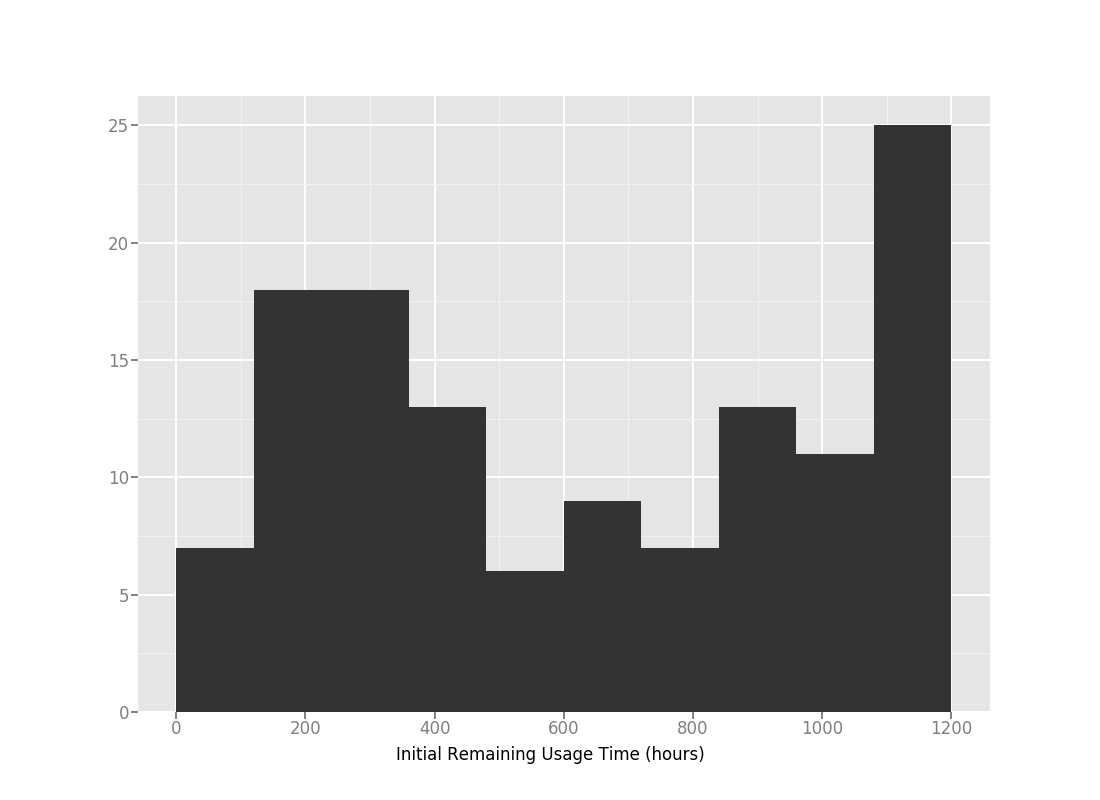
\includegraphics[width=0.5\textwidth]{./../../img/initial_used.png}
    %   \caption{Distribution of Usage Times among resources at the beginning of the planning horizon}
    %   \label{fig:histogramUsage}
    % \end{figure}

% \section{Heuristics}

\section{Results}
  \label{sec:results}

  \subsection{Numerical tests}
    \label{sec:tests}


    All tests were run on a 64 bit Ubuntu 16.04 workstation with 16GB of RAM and Intel i7-6700HQ CPU \@ 2.60GHz x 8 processor.
    Several experiments were done with the MIP formulation on problem instances presented in table \ref{tab:instance}.

    Table \ref{tab:summary} gives an overview of the obtained results. As can be seen, smaller instances are solved up to optimality while medium-size ones are stopped after one hour.

    For this calculation, both weights on the objective function were set at 1. A sensibility analysis of these two parameters is provided in section \ref{sec:multi}.

    \begin{table}
    \begin{center}

    \begin{tabular}{lrrrr}
\toprule
   id &  objective &  gap (\%) &  time (s) &  bound \\
\midrule
 2321 &      139.0 &      0.7 &       500 &  138.0 \\
 2127 &       83.0 &      1.2 &      3600 &   82.0 \\
 2259 &      149.0 &      6.1 &      3600 &  139.9 \\
 1813 &       83.0 &      0.0 &      3600 &   83.0 \\
 1817 &       84.0 &      2.6 &      3600 &   81.8 \\
 1331 &       63.0 &      0.0 &      3600 &   63.0 \\
 1334 &       63.0 &      1.6 &      3600 &   62.0 \\
\bottomrule
\end{tabular}


    \caption{Information on the solution of each tested instance: "id" is the instance identifier; "objective" is the value of the objective function; "gap" is the percentage gap between the integer solution and the linear relaxation; "time (s)" is the solution time or 3600; and "bound" is the greatest lower bound found from the linear relaxation.}
    \vspace{-0.5cm}
    \label{tab:summary}
    \end{center}
    \end{table}

    Table \ref{tab:results} shows the details of the solving process for each instance. As it can be seen, cuts do not improve significantly the relaxation (the value of "bound cuts" is very close to the root solution). In fact, the original linear relaxation (root) is quite similar to the final lower bound (bound). This suggests that further improvement in modelization would help to reduce the gap faster.

    An example of a tighter modelization could be to replace the constraints that count the remaining usage time and elapsed time for tighter equivalents.
    
    The greatest number of cuts used was of 'Implied bound' and 'Mixed integer rounding', depending on the instance. Since these are two generic-type cuts, it can be concluded that the solver has not detected any particular structure as part of this problem.

    \begin{table}
    \begin{center}

    \begin{tabular}{lrrrrr}
\toprule
   id &  root &  b. cuts &  bound &  cuts (\#) &  cuts (s) \\
\midrule
 I\_0 &  56.0 &     61.9 &   62.0 &         37 &       0.7 \\
 I\_1 &  56.0 &     63.0 &   63.0 &        494 &      20.3 \\
 I\_2 &  61.4 &     62.0 &   62.0 &        982 &      25.6 \\
 I\_3 &  60.6 &     60.7 &   61.7 &       1149 &      42.5 \\
 I\_4 &  81.8 &     82.0 &   82.0 &         49 &       0.9 \\
 I\_5 &  82.0 &     83.0 &   83.0 &        752 &      20.3 \\
 I\_6 &  81.4 &     82.0 &   82.0 &        862 &      68.8 \\
 I\_7 &  80.6 &     80.7 &   81.8 &       1489 &      65.1 \\
 I\_8 & 136.8 &    137.8 &  139.0 &        285 &       6.9 \\
 I\_9 & 138.2 &    139.6 &  139.9 &       1157 &     310.8 \\
\bottomrule
\end{tabular}


    \caption{Solution details on the progress of the lower bound: "id" is the name of the instance; "root" is the relaxation before cuts; "b. cuts is the relaxation after the cuts; "bound" is the relaxation at the time limit; "cuts (\#)" is the number of cuts; and "cuts (s)" is the time the cuts took in seconds.}
    \vspace{-0.5cm}
    \label{tab:results}
    \end{center}
    \end{table}

    Table \ref{tab:results2} shows the progress of the integer solution for each instance. For more detail on this progress, figure \ref{fig:progress} shows an example of progress for instance with id=I\_7. It can be seen that initial solutions are quite far from the optimal ones due to the use of heuristics at the beginning of the solving process. In fact, for two rather small instances the solver was able to find an optimal solution before starting to branch.

    The obtained results show that the branching is not providing much improvement in increasing the lower bound or finding better integer solutions. The quantity of symmetries in the model, represented as candidates for each task, could be a reason the difficulty in solving large instances. It may exist a very large number of possible candidates to be potentially assigned for each task with respect to the requirements of resources for each task. This reduces the branching capacity of the solver, which tries to explore many nodes that are almost equivalent in reality.

    An example of an alternative to break these symmetries could be to slightly change the objective function so it can measure more gradually the smoothness of the objective and help get better bounds. Another alternative could be to assign priorities to some combinations of resource-task or to limit the number of candidates that can be assigned to each task by some heuristic that clusters resources with tasks. Finally, arbitrarily preassigning (fixing) the final state (in terms of remaining usage time) to each resource could also help break those symmetries without important loss on the objective function value.

    \begin{table}
    \begin{center}

    \begin{tabular}{lrrr}
\toprule
   id &  first &  sol. cuts &  last \\
\midrule
 I\_0 & 1550.0 &       62.0 &  62.0 \\
 I\_1 & 1558.0 &       99.0 &  63.0 \\
 I\_2 & 1532.0 &       67.0 &  63.0 \\
 I\_3 & 1532.0 &      137.0 &  64.0 \\
 I\_4 & 1544.0 &       82.0 &  82.0 \\
 I\_5 & 1552.0 &      847.0 &  83.0 \\
 I\_6 & 1552.0 &       95.0 &  83.0 \\
 I\_7 & 1552.0 &      856.0 &  84.0 \\
 I\_8 & 1594.0 &      147.0 & 139.0 \\
 I\_9 &  149.0 &        - & 149.0 \\
\bottomrule
\end{tabular}


    \caption{Solution details on the progress of the integer solution: "id" is the name of the instance; "first" is the first solution integer found; "sol. cuts" is the solution after the cuts; "last" is the last solution found at the time limit.}
    \vspace{-0.5cm}
    \label{tab:results2}
    \end{center}
    \end{table}

    \begin{figure}
      \centering
        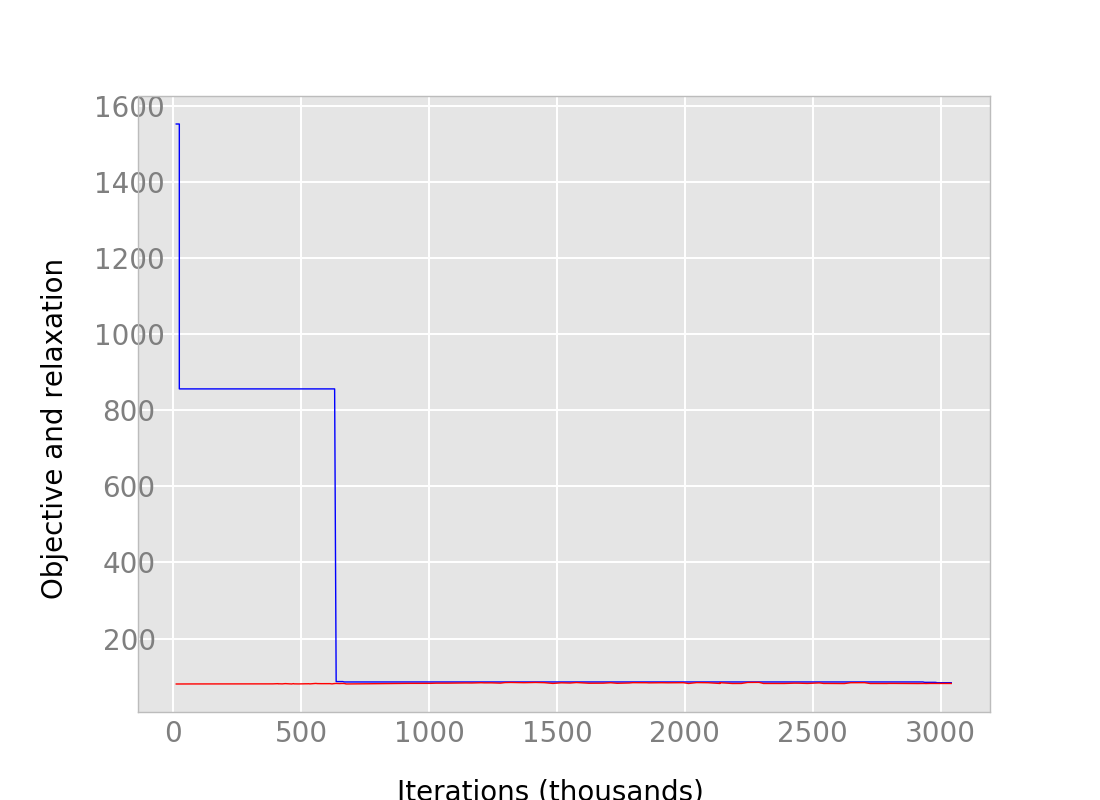
\includegraphics[width=0.5\textwidth]{./../../img/progress.png}
      \caption{Solving progress of the integer solution (in blue) and the lower bound (red) along the solver iterations (x axis). Instance id=I\_7.}
      \label{fig:progress}
    \end{figure}

    Figures \ref{fig:num-maintenances} and \ref{fig:num-unavailables} show an example distribution of maintenance operations and unavailable numbers of resources per period, respectively.

    \begin{figure}
      \centering
        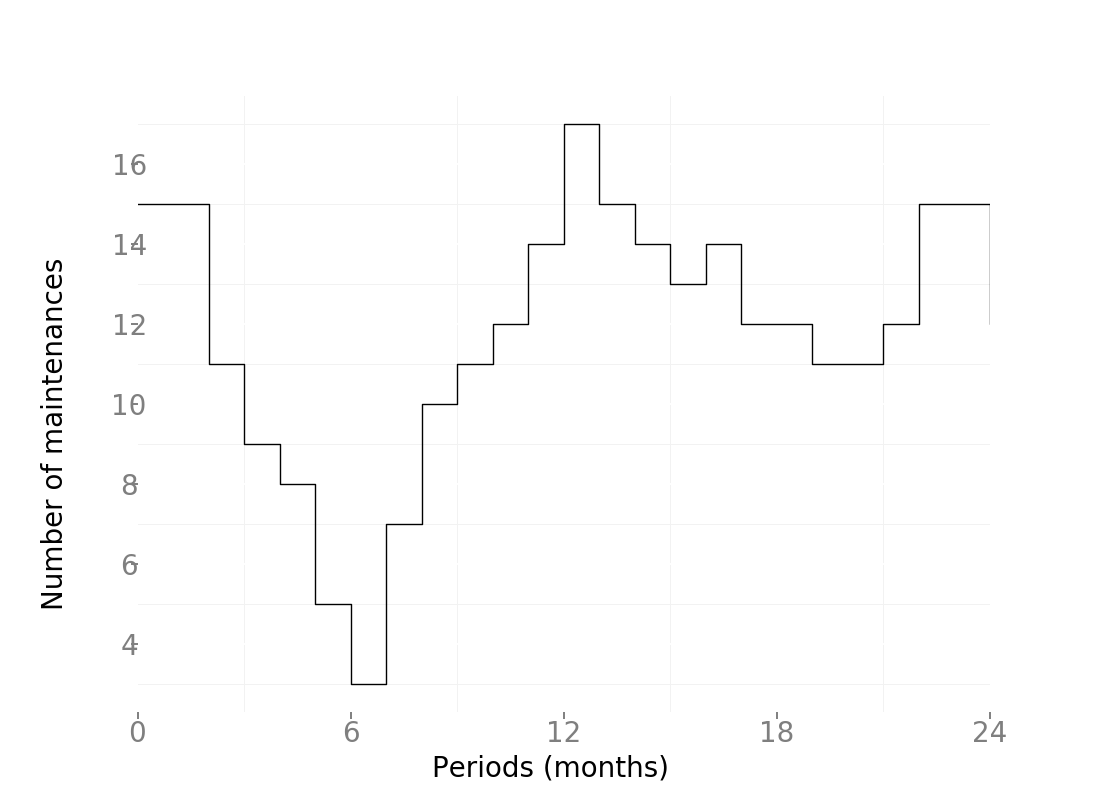
\includegraphics[width=0.5\textwidth]{./../../img/num-maintenances.png}
      \caption{Solution for instance id=I\_7: number of resources under maintenance at each period.}
      \label{fig:num-maintenances}
    \end{figure}

    \begin{figure}
      \centering
        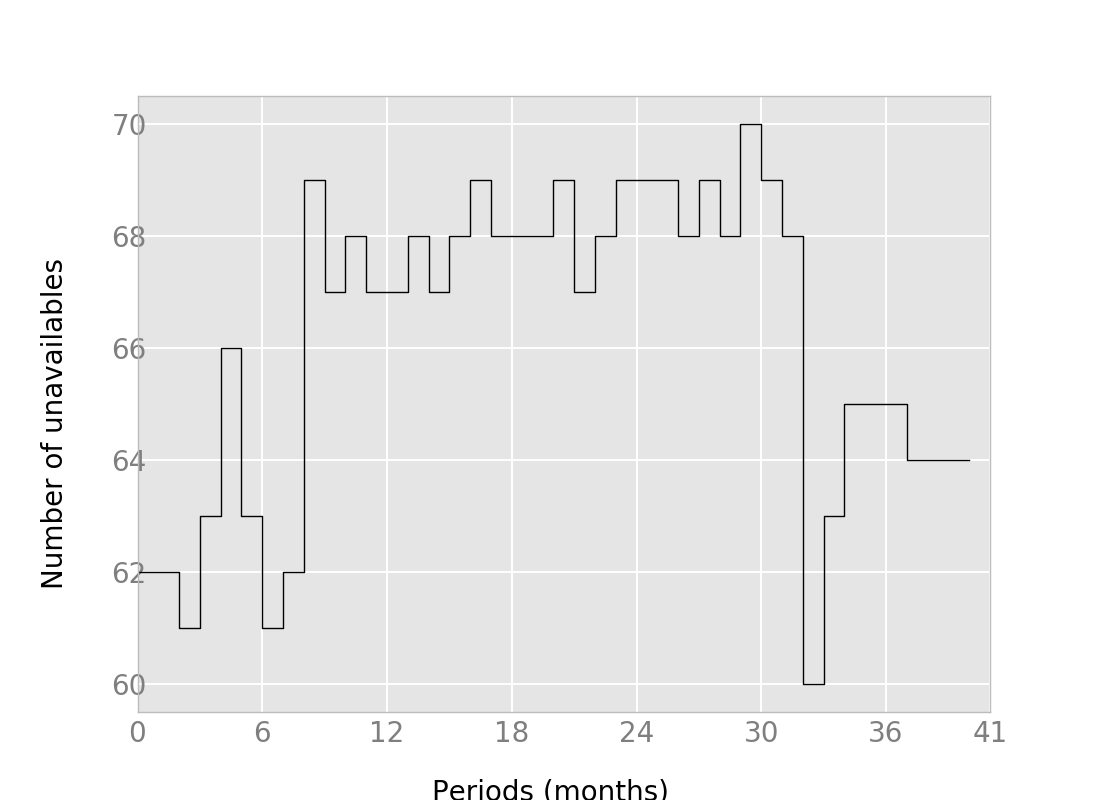
\includegraphics[width=0.5\textwidth]{./../../img/num-unavailables.png}
      \caption{Solution for instance id=I\_7: number of unavailable resources at each period.}
      \label{fig:num-unavailables}
    \end{figure}


  \subsection{Bi-objective analysis}
  \label{sec:multi}

    The further calculation was done in order to analyze the impact of the weights $W_1$ and $W_2$ on the solution. In it, both weights were changed between 0 and 1 with pace of 0.1 under the condition that $W_1 + W_2 = 1 $. This was done for all previously defined instances.

    Table \ref{tab:multmultiobj} presents the obtained results of this analysis. It can be seen that all instances have a small number of non-dominated solutions.

    \begin{table}[h]
    \begin{center}

    \begin{tabular}{lrll}
\toprule
   id &  \# points &      First &       Last \\
\midrule
 I\_0 &          3 &   (18, 45) &   (15, 47) \\
 I\_1 &          3 &   (20, 46) &   (15, 48) \\
 I\_2 &          2 &   (16, 47) &   (15, 48) \\
 I\_3 &          3 &   (19, 45) &   (15, 49) \\
 I\_4 &          3 &   (18, 65) &   (15, 67) \\
 I\_5 &          3 &   (20, 66) &   (15, 68) \\
 I\_6 &          2 &   (16, 67) &   (15, 68) \\
 I\_7 &          4 &   (19, 66) &   (16, 69) \\
 I\_8 &          2 &  (21, 118) &  (18, 121) \\
 I\_9 &          3 &  (24, 121) &  (20, 122) \\
\bottomrule
\end{tabular}


    \caption{Non-dominated points found on each instance after 3600 seconds. All instances were analyzed: "First" and "Last" indicate the two extremes of the calculated Pareto frontier; "\# points" indicates the number of Pareto optimal points found. Not all experiments were solved up to optimality.}
    \vspace{-0.5cm}
    \label{tab:multmultiobj}
    \end{center}
    \end{table}

    More particularly, an individual instance was analyzed, where an optimal solution was found in each experiment.
    Table \ref{tab:multiobj} shows the obtained results. The instance used consisted of 21 periods and 10 tasks corresponding to instance with id=I\_5.

    For all solved instances, a small number of non dominated solutions was observed.
    \begin{table}[h]
    \begin{center}

    \begin{tabular}{lrrrr}
\toprule
 exp &  maint &  unavailable &  $w_1$ &  $w_2$ \\
\midrule
 W00 &     20 &           66 &    0.0 &    1.0 \\
 W01 &     20 &           66 &    0.1 &    0.9 \\
 W02 &     20 &           66 &    0.2 &    0.8 \\
 W03 &     16 &           67 &    0.3 &    0.7 \\
 W04 &     16 &           67 &    0.4 &    0.6 \\
 W05 &     15 &           68 &    0.5 &    0.5 \\
 W06 &     15 &           68 &    0.6 &    0.4 \\
 W07 &     15 &           70 &    0.7 &    0.3 \\
 W08 &     15 &           68 &    0.8 &    0.2 \\
 W09 &     15 &           69 &    0.9 &    0.1 \\
 W10 &     15 &           69 &    1.0 &    0.0 \\
\bottomrule
\end{tabular}


    \caption{Values of $u_{max}$ (unavailable) and $m_{max}$ (maint) for different combinations of $W_{1}$ and $W_{2}$. Instance id=I\_5. All experiments were solved to optimality.}
    \vspace{-0.5cm}
    \label{tab:multiobj}
    \end{center}
    \end{table}

    \begin{figure}
      \centering
        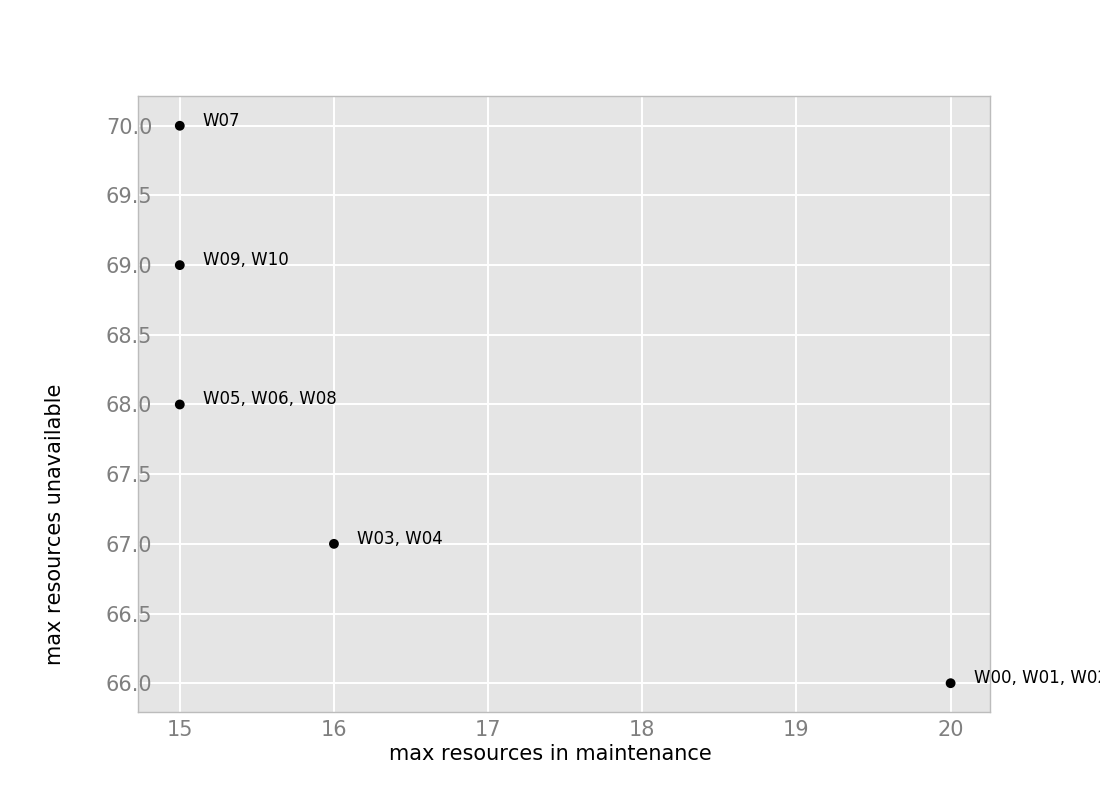
\includegraphics[width=0.5\textwidth]{./../../img/multiobjective.png}
      \caption{Pareto diagram for instance id=I\_5.}
      \label{fig:pareto}
    \end{figure}

\section{Conclusions and further work}
  \label{sec:conclusions}

  This paper proposed a new MIP formulation to address a specific FMP with an heterogeneous fleet of aircraft.
  Two objective functions were chosen to address the French Air Force requirements.
  The first one was to smooth maintenance operations and the second one was to increase aircraft availability.
  The characteristics of MIP convergence were analyzed on real-world instances.
  Mono-objective problem instances were solved to optimality for medium size instances. Then, exact Pareto frontiers for bi-objective formulation were calculated for these instances. 
  The use of these two objectives does not lead to the same optimal solution but very good compromise solutions can be found due to the bi-objective optimization.
  For larger instances, difficulties in finding optimal solutions occurred because of multiple symmetries and a poor quality of MIP generic primal heuristics.

  The first perspective is to improve the resolution of large size instances. Heuristics could be implemented, but also mathematical programming can be improved with symmetry breaking or MIP reformulations. 
  For the bi-objective optimization for large size instances, more advanced bi-objective methods such as $\epsilon$-constraints or Two-Phases-Method should be investigated for the computation of larger Pareto frontiers.
  Lastly, additional constraints from the real world application can be incorporated in the model.

\bibliographystyle{dcu}
\bibliography{./../biblio/MFMP}

\end{document}